% tikz-diagram — a single-file project with one TikZ diagram. It compiles as-is.
\documentclass[11pt, a4paper]{article}

\usepackage[T1]{fontenc}
\usepackage[utf8]{inputenc}
\usepackage{tikz}
\usetikzlibrary{arrows.meta, positioning, shapes.geometric}

\title{A TikZ Diagram}
\author{Your Name}
\date{\today}

\begin{document}

\maketitle

\section{A flow diagram}
Figure~\ref{fig:flow} is drawn entirely in TikZ: nodes are placed relative to
one another and joined with arrows, so moving one node moves the diagram with it.

\begin{figure}[ht]
  \centering
  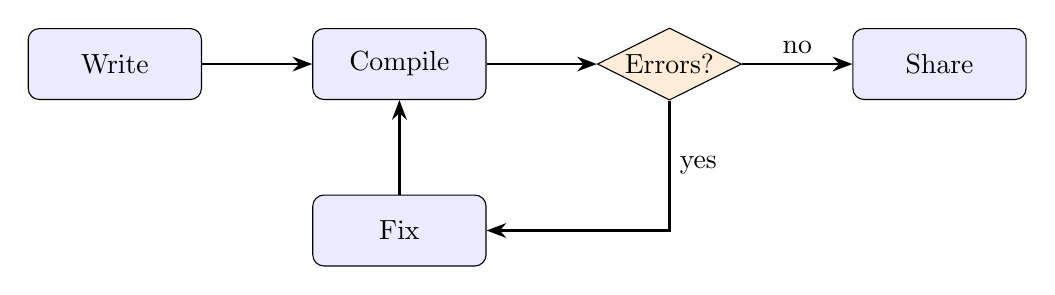
\begin{tikzpicture}[
      node distance = 12mm and 14mm,
      box/.style    = {draw, rounded corners, minimum width=22mm, minimum height=9mm, fill=blue!8},
      choice/.style = {draw, diamond, aspect=2, inner sep=1pt, fill=orange!15},
      arrow/.style  = {-{Stealth[length=2.5mm]}, thick}
    ]
    \node[box]                            (write)   {Write};
    \node[box,    right=of write]         (compile) {Compile};
    \node[choice, right=of compile]       (ok)      {Errors?};
    \node[box,    right=of ok]            (share)   {Share};
    \node[box,    below=of compile]       (fix)     {Fix};

    \draw[arrow] (write)   -- (compile);
    \draw[arrow] (compile) -- (ok);
    \draw[arrow] (ok)      -- node[above] {no} (share);
    \draw[arrow] (ok)      |- node[pos=0.25, right] {yes} (fix);
    \draw[arrow] (fix)     -- (compile);
  \end{tikzpicture}
  \caption{Write, compile, fix, repeat.}
  \label{fig:flow}
\end{figure}

\section{A plot}
TikZ also draws figures from formulas, with no data file needed:

\begin{center}
  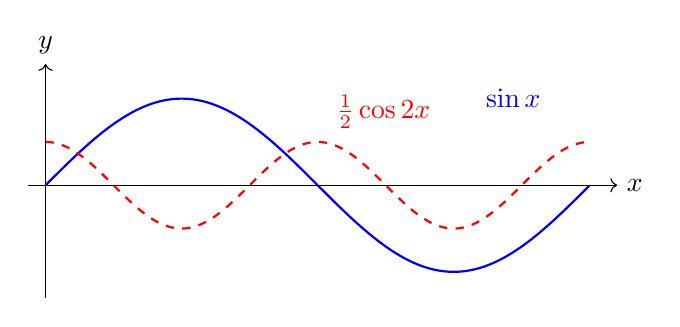
\begin{tikzpicture}[scale=1.1]
    \draw[->] (-0.2,0) -- (6.6,0) node[right] {$x$};
    \draw[->] (0,-1.3) -- (0,1.4) node[above] {$y$};
    \draw[thick, blue, domain=0:6.28, samples=100, smooth]
      plot (\x, {sin(\x r)});
    \draw[thick, red, dashed, domain=0:6.28, samples=100, smooth]
      plot (\x, {0.5*cos(2*\x r)});
    \node[blue] at (5.4,1.0) {$\sin x$};
    \node[red]  at (3.9,0.85) {$\frac{1}{2}\cos 2x$};
  \end{tikzpicture}
\end{center}

\end{document}
